\section{System Model}\label{sec:system_model}
In this section, we explain GPU task model on this paper while we discuss the gpu scheduling question and prior work.
Next, we make available limitation for clearing the implementation of no patched gpu scheduling.
This paper focus on a system composed of multiple GPU and multi-core CPU.

\subsection{GPU Task Model}
When using GPU in general-purpose way, CUDA and OpenCL can use much.
In this paper, we only use CUDA, but it is possible the same approach even OpenCL.

GPU applications use a set of the API supported by the system,
typically talking the following steps.
(i) create GPU context (\textit{cuCtxCreate}), 
(ii) allocate space to device memory (\textit{cuMemAlloc}), 
(iii) The data and the GPU kernel are copied to the allocated device memory space from host memory (\textit{cuMemcpyHtoD}), 
(iv) Launch the GPU kernele (\textit{cuLaunchGrid}), 
(v) The GPU task is synchronized to the GPU kernel (\textit{cuCtxSynchronize}), 
(vi) The resultant data transfer to host memory from device memory (\textit{cuMemcpyDtoH}), 
(vii) release allocated memory space and context (\textit{cuMemFree, cuModuleUnload, cuCtxDestroy}).

We define a GPU task which is to execute the GPU using above API flow,
and define a GPU kernel that is unit of processing to executed on the GPU side.

%我々は本稿においては、GPU実行が少しでも含まれるプロセスであり、ある事柄を成し遂げる一つの単位をアプリケーションとする。 (e.g. pedestrian detection application).
%またこの一連の流れによってGPUを実行する1プロセスをGPUタスクとし、
%GPU側で実行されるカーネルをGPUカーネルと定義する。

\subsection{GPU Scheduling}
Real-time OS (RTOS) is a lot of research\cite{spring, redline,itron,rk} has been conducted for a long time.
In among them have also been many studies\cite{prk,rtai,yodaiken1999rtlinux,litmus,kato:loadable} real-time OS, which is based on the Linux.
%リアルタイムOSは古来より多くの研究\cite{spring,redline,itron,rk}が行われてきている。
%LinuxをベースとしたリアルタイムOSとしても数多く研究\cite{prk,rtai,yodaiken1999rtlinux,litmus,kato:loadable}されている。
%GPUを利用可能な環境はWindows, Mac OS, Linuxと限られており、リアルタイムという性質を追求するためにはLinuxの利用が最適であるため、今回我々はlinuxを利用する。
OS available the GPU is limited to Windows, Mac OS and Linux,
we selected Linux in order to achieve real-time on GPU environments.

Requirement that the scheduler the minimum required in carrying to realize the real-time multi-core environment is the following two:
%マルチコア環境でリアルタイムを実現するにあたりスケジューラが最低限必要とする要件は以下の2つである.
\begin{itemize}
\item To use resources according to order.
%.The mechanisms is resources that are available to the specified order
%u指れた順番でリソースが利用可能なこと
\item To limit the use of the shared resource
\end{itemize}
The basic approach to satisfy the first is priority-based scheduling (e.g. Rate-Monotonic\cite{sched:rm} and Earliest Deadline First\cite{sched:edf}) with technique to prevent priority inversion,
and the second is resource reservation based scheduling (e.g. Constant Bandwidth Server\cite{rr:cbs}, Total Bandwidth Server\cite{rr:tbs2}).
%これらを満たすための基本的なアプローチとして,一つ目は優先度ベースのスケジューリング (e.g. Rate-monotonic, Earliest deadline first),
%2つ目は,リソースリザベーションベースのスケジューリング (e.g. CBS, TBS, credit)が用いられる.
The GPU to handle the data transfer bandwidth and the processing core as a shared resource,
it is necessary to satisfy the two requirements similar to above multicore environment.
%GPUはデータ転送帯域,プロセッシングコアの2つを共有リソースとして扱う必要性があり,上記マルチコア環境と同様に2つの要件を満たす必要がある.
%Therefore, in the system of including GPU is 
%そのためGPUが含まれるシステムにおいても,リアルタイムを実現するためには上記二点を達成できればよい.
Our previous working only to scheduling GPU accesses.
However, GPU kernel is driven by API is issued GPU task, to truly support  the real-time scheduling, it is need to schedule GPU task; therefore, for realized real-time GPU, framework need to have CPU's priority-based scheduler, GPU's priority-based schedulera and restrict GPU resource by resource reservation mechanisms.
%我々がこれまで取り組んできたGPUリソースマネージメントに関する研究では,
%GPUへのアクセスのみをスケジューリングしてきた.
%しかしながらGPUカーネルはGPUタスクから発行されるAPIを起点に動作していることから,
%真にリアルタイムスケジューリングを適応するためには,GPUタスク自体のスケジューリングを行う必要がある.
%したがって,GPUをリアルタイムにスケジューリングするために必要なメカニズムは,
%CPUの優先度ベーススケジューラ,GPUの優先度ベーススケジューラ,リソースリザベーションによるGPUリソース制限である.
Recently, GPUSync is to work the above interdependence of CPU scheduler and GPU scheduler.
%最近ではGPUSyncが上記のCPUスケジューラとGPUスケジューラの相互依存について取り組んでいる.
%GPUSync needs to install by patch because it depends to $LITMUS^RT$.

%しかし,GPUSyncは$LITMUS^RT$に依存しており,パッチによるインストレーションを必要とする.
%Section~\ref{sec:intro}で述べたとおり,カーネルにパッチを当てる作業は大きな負担になる.
GPUs have some problem on using realtime, except that scheduling mechanisms.
%GPUのリアルタイム活用にはスケジューリングメカニズム以外の面でも多くの問題がある.
GPUs runtime environments are blackbox mechanisms results from GPU environments are provided only GPU vendors and these environments are closed-source.
%まずGPUの実行環境がベンダーから提供されるのみであり,クローズドソースになっていることからブラックボックスであることである.
TimeGraph, Gdev and RGEM are solved this problem by ensuring transparency using reverse engineering and open-source driver.
%本問題についてはTIMEGRAPH,GDEV,RGEMではリバースエンジニアリングとオープンソースドライバによって透明性を確保している.
GPUSync is solved this problem too by GPU runtime resource management is disabled through the runtime access to single.
%GPUSyncではランタイムドライバへのアクセスを単一に制限することで,ランタイムドライバが行う資源管理をスルーしている.

The other problem occurs by non-preemptive GPU executions and non-preemptive data transfers.
several researchs\cite{} realize implovement the responce time by preventing divides the kernel overrun.
%GPUの実行やデータ転送がノンプリエンプティブであることも大きな問題だ.いくつかの研究\cite{}ではカーネルを分割することで,
%ノンプリエンプティブに起因するオーバランを防ぎ,レスポンスタイムの向上を実現している.

As these core problems are headling to solve, however, real-time GPU is experimental-phase since have problem for practical realized.
%このようにいくつかのコアな問題は解決に近づいているが,未だリアルタイムGPUは実験フェーズであり,実用化に向けるには問題が存在している.
The most difficult problem is self-supension due to GPU is treated as a I/O device.
GPU task to suspended themselfs until it receives the results from issuing the processing to GPU, referred to as self-suspension.
%GPUを完全にリアルタイムに扱うことができないもっとも困難な問題は,GPUがI/Oデバイスとして扱われることに起因する.
%GPUに処理を発行し,結果を受け取るまでの間,発行したタスクは自らサスペンドする.
The self-suspension has been proven as a cause the NP-HARD problem in previous work\cite{self-sus:1,self-sus:2},
several researchs\cite{chattopadhyay2014limited, kim2013segment} are working on the scheduling analysis for self-suspension task, but it has not been solved yet to complete.

Hence scheduling framework for the expansion and installation to aim in this study and easy is useful,
it is argued that there is a demand.

%このself-suspensionはこれまでの研究\cite{self-sus:1,self-sus:2}でNP-HARDな問題を発生させるとして証明されており,
%これまでも多くの研究が執り行われている\cite{chattopadhyay2014limited,kim2013segment}が,実用レベルでは未だ解決されていない問題である.

%そのため本研究で目指すような拡張,インストールを容易とするスケジューリングフレームワーク実験レベル,実用レベルの両者において有用であり,需要が発生すると推測する.

\if 0
\textbf{Scheduling policies:}
We discuss the scheduling policies to be equipped as the scheduling foundation.
%ここでは上記スケジューリング基盤として備えるべきスケジューリングポリシーについて議論する。
Generaly, CPU task is sufficient that can priority schedling in the real-time systems.
Priority scheduling are two main categories, that are Fixed Prioriry scheduling (e.g. ratemonotonic, deadline monotonic) and Dinamic Priority scheduling (e.g. Earliest Deadline First:EDF).

%CPU側で動作するタスクに関してはリアルタイムなシステムにおいては、優先度スケジューリング且ができていればよい。
%固定優先度方式としてDeadline-Monotonic (DM)\cite{sched:dm}やRate-Monotonic (RM)\cite{sched:rm}などがあり、
%動的優先度方式としてEarist deadline first (EDF) などがある。

GPU kernele execution is to inconvenience in the prioriry-based scheduling.
GPU kernek is including GPU task, therefore, priority inversion is happend in the case of different the GPU kernel priority and the GPU task kernel priority.
Thus basically, GPU kernel scheduling is appropriate to follow the priority of the process.
Additionally, scheduler need each GPU tasks QoS management.

%GPUカーネルの実行に関しては優先度ベースなスケジューリングでは不都合が生じる。
%GPUカーネルはGPUタスクに含まれるものである。
%そのためGPUカーネルの優先度とGPUタスクの優先度が異なるケースは、その時点でGPUタスクの優先度逆転が発生する。
%したがって、GPUカーネルスケジューリングはプロセスのスケジューリングに沿って実行するのが適正であり、
%それに加えて必要なのが各GPUタスクごとのGPUリクエストに対するQoSを担保することである。

%QoSを担保する方法としてこれまでリソースリザベーションベースのスケジューリングポリシーが提案\cite{gdev,cbs,tbs}されてきており、
The resource reservation-based scheduling policy has been proposed\cite{gdev,cbs,tbs} as a method to guarantee QoS.
This paper adopt the BAND scheduling that gave a certain defree of success in QoS collateral in Gdev.
%本論文ではGdevでGPUのQoS担保に一定の成果を挙げたBANDスケジューリングを利用する。

\fi

\textbf{kernel free scheduler:}
To achieve "kernel free", we must not to modify the kernel code and the device driver code.
RGEM does scheduling on the only user-space, this is realized priority-based sheduling by using is IPC (Inter Process Communication) privided by POSIX.

GPU scheduling does synchronization based scheduling,
however, RGEM is to depends on the runtime software synchronization.
%RGEMはユーザスペースのみでGPUカーネルラウンチのスケジューリングを行っている。
%GPUタスク間でPOSIXによって提供されるIPCを用いてタスク間の協調を行い、優先度ベースでのスケジューリングを実現している。
%GPUのスケジューリングは同期ベースなスケジューリングを行うが、RGEMでは同期の取得をランタイムに依存している。

%同期の取得を行うように変更するためにカーネルスペースからのアプローチが必須である。
Gdev has been achieved independs synchronization mechanisms on the proprietary software, need to modify the kernel modification.
The challenge is realize independs synchronization mechanisms by kernel free aproach.

%Gdevではカーネルスペースからのアプローチを行っているが、
%同期の取得のためにカーネルへの変更を含んでいるため、
%同期の取得をノーパッチで行うことが大きな課題である。

\textbf{GPU Synchronization:}
%GPUを利用するシステムのようなヘテロジニアス且つメモリを共有しない場合に大きな課題となるのが同期である
The synchronization matters for GPU system such as heterogeneous platoform.
Furthermore, as mentioned we need to achieve the independs synchronization mechanisms by the kernel free aproach.

GPU have two different synchronization techniques.
The first techniques memory map based synchronization is called FENCE, 
it sends GPU commands after the command to take action, then GPUs microcontrollers will write the any value to memory-mapped space after action is completed.
GPU task monitors it mapped space value using such as polling, therefore task has an exclusive CPU resource, but response time will be the fastest.
The other one is interrupts based synchronization is called NOTIFY,
it sends GPU commands similar to FENCE, then GPUs microcontrollers will rise the interrupt and write any value to GPU I/O registers.
GPU task is suspending until interrupt, therefore task is able to share the CPU resources with other tasks, but response time will be the slow.
Detailed architecture is omitted in this paper, it has been described in the previous documents\cite{kato:timegraph,kato:gdev,fujii:apsys2013}.

NOTIFYによる同期を実現するためには,割込みを取得しそれがどのコンテキストから発行されたものかを識別しなければならない.
FENCEによる同期を実現するためには,コマンドを送信できるようにしなければならない.

Gdev use both techniques that are NOTIFY and FENCE for wakeup the waiting task, NOTIFY is used by scheduler, FENCE is used by kernel synchronization.
Gdev's synchronization implementation is the addtional commands sends to GPU and the modification of device driver's interrupt handler.
GPUSync use NOTIFY techniques by using tasklet intercept. 
tasklet is linux's soft-irq implementation.
GPUSync identify the interrupt that is issued which kernel by callback pointer with a tasklet.


%本稿で対象とするプラットフォームでは、複数のGPUタスクが存在し、複数のGPUカーネルが同一タスクに存在することを想定している。
%そのため複数のGPUカーネルと一般的に同期に利用されるCUDA APIの$cuCtxSynchronize()$の回数は一対一で対応付けされずに、
%複数のGPUカーネルの発行を一度の$cuCtxSynchronize()$によって同期する可能性がある。
%そのため、$cuCtxSynchronize()$を用いた同期ベースなスケジューリングを行うにあたり、各GPUカーネルの終了と同期のために、アプリケーション自体の変更を必要とするため好ましくない。

%本問題に対してGPUSyncではNOTIFYに限って対処しており、$LITMUS^{RT}$の拡張という形でLinuxの割込みのbottom-halfであるtaskletをカーネル内部で傍受し、
%コールバック関数の引数のポインタが指すメモリスペースによって、どのGPUからの割込みかを判断している。
\if 0
その手法では、soft-irqを利用しているためレイテンシが大きく、どのカーネルであるかの判断もできない。
GdevではGPUタスクの同期はFENCE、スケジューラの立ち上げはNOTIFYを用いている。
NOTIFYの獲得は、デバイスドライバがカーネルに登録するISRにGdevのコールバック関数を追記することで割込みタイミングを獲得している。
GPUタスクの同期にFENCEを用いている理由としては、あくまでGPUを効率よく扱う点にフォーカスしており、CPU側の処理も含めた効率について考慮していないためである。
ただし,GPUの実行はすべてAPIドリブンであり,CPU側で動作するGPUタスクからGPUカーネルを発行されて実行が行われる.
GPUカーネルの優先度とGPUタスクの優先度が異なるケースはよほど特殊でない限り利用しない(我々の思いつく限り存在しない)ため,
are non-preemptive
カーネル、デバイスドライバの編集無しにスケジューリングするための最も大きな課題は、この同期を獲得し、識別するかといった点である。
\fi

\if 0
本稿で対象とするプラットフォームでは、複数のGPUタスクが存在し、複数のGPUカーネルが同一タスクに存在することを想定している。
そのため複数のGPUカーネルと一般的に同期に利用されるCUDA APIの$cuCtxSynchronize()$の回数は一対一で対応付けされずに、
複数のGPUカーネルの発行を一度の$cuCtxSynchronize()$によって同期する可能性がある。
そのため、$cuCtxSynchronize()$を用いた同期ベースなスケジューリングを行うにあたり、各GPUカーネルの終了と同期のために、アプリケーション自体の変更を必要とするため好ましくない。

本問題に対してGPUSyncではNOTIFYに限って対処しており、$LITMUS^{RT}$の拡張という形でLinuxの割込みのbottom-halfであるtaskletをカーネル内部で傍受し、
コールバック関数の引数のポインタが指すメモリスペースによって、どのGPUからの割込みかを判断している。
その手法では、soft-irqを利用しているためレイテンシが大きく、どのカーネルであるかの判断もできない。
GdevではGPUタスクの同期はFENCE、スケジューラの立ち上げはNOTIFYを用いている。
NOTIFYの獲得は、デバイスドライバがカーネルに登録するISRにGdevのコールバック関数を追記することで割込みタイミングを獲得している。
GPUタスクの同期にFENCEを用いている理由としては、あくまでGPUを効率よく扱う点にフォーカスしており、CPU側の処理も含めた効率について考慮していないためである。
ただし,GPUの実行はすべてAPIドリブンであり,CPU側で動作するGPUタスクからGPUカーネルを発行されて実行が行われる.
GPUカーネルの優先度とGPUタスクの優先度が異なるケースはよほど特殊でない限り利用しない(我々の思いつく限り存在しない)ため,
are non-preemptive
カーネル、デバイスドライバの編集無しにスケジューリングするための最も大きな課題は、この同期を獲得し、識別するかといった点である。
\fi
%GPUの同期は2つの手法がある。
%一つはPollingを用いた方法で本誌ではFENCEと呼ぶ。
%もう一つはInterruptによって同期する方法で本誌ではNOTIFYと呼ぶ。
%これらは両者ともGPUに搭載されたエンジンを用いて行われる。
%GPUには多くのエンジン(マイクロコントローラ)が搭載されている。
%本論文では詳しいアーキテクチャはメインではないので省略するが、詳細は過去の文献\cite{kato:timegraph,fujii:apsys2013}に記載しています。
%このエンジンにはコンテキスト管理用、コマンド受け取り用、データ転送用などが存在している。
%通常、コマンド受け取り用のエンジンが受け取ったコマンドのヘッダから、
%そのコマンドを使用するエンジンへと送信し、処理が行われる。
%この順序はすべてFIFOで行われる。
%FENCEを用いた方式では、まず同期用に仮想アドレス空間にマップされたバッファをGPUメモリに用意する。
%そして、このメモリに値をEngine経由で書き込むためのコマンドを発行する。
%Engineはカーネル実行とメモリ転送終了後に値を書き込むため、
%CPU側でマップされたメモリアドレスをポーリングしながらチェックすれば同期が可能である。
%NOTIFYについてもEngineの機能を利用する。

%タスクはTASK\_INTERRUPTIBLE or TASK\_UNINTERRUPTIBLEにした上でschedule()を呼ぶか、
%waitqueueなどを用いて上記に相当する処理を行いsuspendする。
%そしてEngineから割込みを発生させるコマンドを発行し、割り込みコントローラがそれを獲得、
%GPUドライバが登録した$Interrupt Service Routine$ (ISR) を立ち上げる。
%ISR内では、各割込みに関するステータスをマッピングされたレジスタから読み込み、
%各割込みごとに処理を行う。処理後は割込み完了フラグを書き込み、初期化する。
%Gdevではsynchronization ベースのスケジューリングを行っており、GPUカーネル終了の検知し次のタスクを立ち上げる部分に割込みを用いている。

\if 0
\begin{figure}[t]
\begin{center}
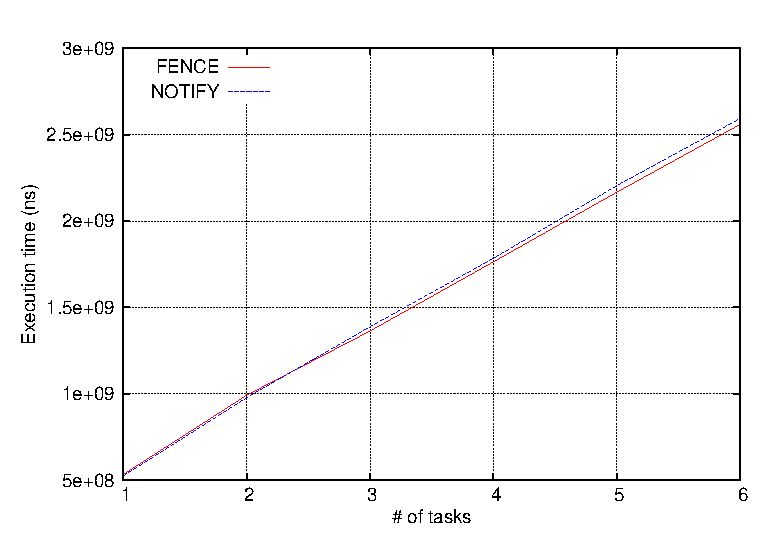
\includegraphics[width=0.35\textwidth]{img/poll_vs_irq}
\caption{FENCE vs NOTIFY}
\end{center}
\label{fig:poll_vs_irq}
\end{figure}
\fi

%二種類の手法が存在する理由としては、FENCEとNOTIFYにそれぞれアドバンテージがあるためである。
%Figure~\ref{fig:poll_vs_irq} shows FENCEを1とした時のNOTIFYのrelative speedである。
%タスクが1つの場合はFENCEがNOTIFYよりも8ms速い結果が出ており、
%タスクが3個に増えた時点でNOTIFYの方が早くなり、タスク6個の時点では33ms速い結果がでている。
%NOTIFYによってタスクがスリープしている間に他のタスクのCPU利用部分が動作することで、
%効率的にGPUタスクが実行できているためである。
%GPUをより効率的に利用するためにはFENCE、NOTIFYをうまく使い分ける必要がある。

